\section{Results}
\label{sec:res}

\subsection{TS Results}

\begin{figure}[h]
    \begin{centering}
        % GNUPLOT: LaTeX picture with Postscript
\begingroup
  \makeatletter
  \providecommand\color[2][]{%
    \GenericError{(gnuplot) \space\space\space\@spaces}{%
      Package color not loaded in conjunction with
      terminal option `colourtext'%
    }{See the gnuplot documentation for explanation.%
    }{Either use 'blacktext' in gnuplot or load the package
      color.sty in LaTeX.}%
    \renewcommand\color[2][]{}%
  }%
  \providecommand\includegraphics[2][]{%
    \GenericError{(gnuplot) \space\space\space\@spaces}{%
      Package graphicx or graphics not loaded%
    }{See the gnuplot documentation for explanation.%
    }{The gnuplot epslatex terminal needs graphicx.sty or graphics.sty.}%
    \renewcommand\includegraphics[2][]{}%
  }%
  \providecommand\rotatebox[2]{#2}%
  \@ifundefined{ifGPcolor}{%
    \newif\ifGPcolor
    \GPcolorfalse
  }{}%
  \@ifundefined{ifGPblacktext}{%
    \newif\ifGPblacktext
    \GPblacktexttrue
  }{}%
  % define a \g@addto@macro without @ in the name:
  \let\gplgaddtomacro\g@addto@macro
  % define empty templates for all commands taking text:
  \gdef\gplbacktext{}%
  \gdef\gplfronttext{}%
  \makeatother
  \ifGPblacktext
    % no textcolor at all
    \def\colorrgb#1{}%
    \def\colorgray#1{}%
  \else
    % gray or color?
    \ifGPcolor
      \def\colorrgb#1{\color[rgb]{#1}}%
      \def\colorgray#1{\color[gray]{#1}}%
      \expandafter\def\csname LTw\endcsname{\color{white}}%
      \expandafter\def\csname LTb\endcsname{\color{black}}%
      \expandafter\def\csname LTa\endcsname{\color{black}}%
      \expandafter\def\csname LT0\endcsname{\color[rgb]{1,0,0}}%
      \expandafter\def\csname LT1\endcsname{\color[rgb]{0,1,0}}%
      \expandafter\def\csname LT2\endcsname{\color[rgb]{0,0,1}}%
      \expandafter\def\csname LT3\endcsname{\color[rgb]{1,0,1}}%
      \expandafter\def\csname LT4\endcsname{\color[rgb]{0,1,1}}%
      \expandafter\def\csname LT5\endcsname{\color[rgb]{1,1,0}}%
      \expandafter\def\csname LT6\endcsname{\color[rgb]{0,0,0}}%
      \expandafter\def\csname LT7\endcsname{\color[rgb]{1,0.3,0}}%
      \expandafter\def\csname LT8\endcsname{\color[rgb]{0.5,0.5,0.5}}%
    \else
      % gray
      \def\colorrgb#1{\color{black}}%
      \def\colorgray#1{\color[gray]{#1}}%
      \expandafter\def\csname LTw\endcsname{\color{white}}%
      \expandafter\def\csname LTb\endcsname{\color{black}}%
      \expandafter\def\csname LTa\endcsname{\color{black}}%
      \expandafter\def\csname LT0\endcsname{\color{black}}%
      \expandafter\def\csname LT1\endcsname{\color{black}}%
      \expandafter\def\csname LT2\endcsname{\color{black}}%
      \expandafter\def\csname LT3\endcsname{\color{black}}%
      \expandafter\def\csname LT4\endcsname{\color{black}}%
      \expandafter\def\csname LT5\endcsname{\color{black}}%
      \expandafter\def\csname LT6\endcsname{\color{black}}%
      \expandafter\def\csname LT7\endcsname{\color{black}}%
      \expandafter\def\csname LT8\endcsname{\color{black}}%
    \fi
  \fi
  \setlength{\unitlength}{0.0500bp}%
  \begin{picture}(5040.00,3528.00)%
    \gplgaddtomacro\gplbacktext{%
      \csname LTb\endcsname%
      \put(1078,704){\makebox(0,0)[r]{\strut{} 0.92}}%
      \put(1078,988){\makebox(0,0)[r]{\strut{} 0.94}}%
      \put(1078,1273){\makebox(0,0)[r]{\strut{} 0.96}}%
      \put(1078,1557){\makebox(0,0)[r]{\strut{} 0.98}}%
      \put(1078,1841){\makebox(0,0)[r]{\strut{} 1}}%
      \put(1078,2126){\makebox(0,0)[r]{\strut{} 1.02}}%
      \put(1078,2410){\makebox(0,0)[r]{\strut{} 1.04}}%
      \put(1078,2694){\makebox(0,0)[r]{\strut{} 1.06}}%
      \put(1078,2979){\makebox(0,0)[r]{\strut{} 1.08}}%
      \put(1078,3263){\makebox(0,0)[r]{\strut{} 1.1}}%
      \put(1591,484){\makebox(0,0){\strut{}2}}%
      \put(1973,484){\makebox(0,0){\strut{}4}}%
      \put(2354,484){\makebox(0,0){\strut{}6}}%
      \put(2736,484){\makebox(0,0){\strut{}8}}%
      \put(3117,484){\makebox(0,0){\strut{}10}}%
      \put(3499,484){\makebox(0,0){\strut{}12}}%
      \put(3880,484){\makebox(0,0){\strut{}14}}%
      \put(4262,484){\makebox(0,0){\strut{}16}}%
      \put(176,1983){\rotatebox{-270}{\makebox(0,0){\strut{}Speedup}}}%
      \put(2926,154){\makebox(0,0){\strut{}Distance}}%
    }%
    \gplgaddtomacro\gplfronttext{%
      \csname LTb\endcsname%
      \put(2197,3090){\makebox(0,0)[l]{\strut{}Degree = 1}}%
      \csname LTb\endcsname%
      \put(2197,2870){\makebox(0,0)[l]{\strut{}Degree = 2}}%
      \csname LTb\endcsname%
      \put(2197,2650){\makebox(0,0)[l]{\strut{}Degree = 3}}%
      \csname LTb\endcsname%
      \put(2197,2430){\makebox(0,0)[l]{\strut{}Degree = 4}}%
    }%
    \gplbacktext
    \put(0,0){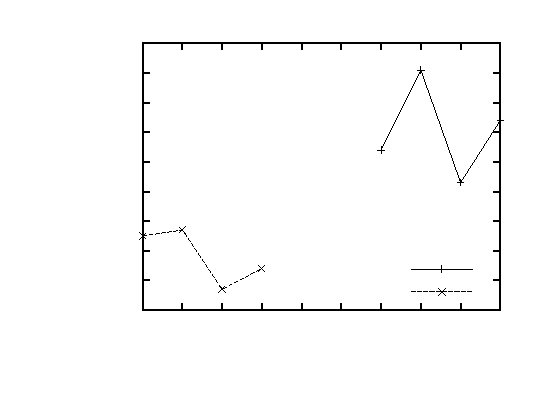
\includegraphics{tagged-sequential-plot}}%
    \gplfronttext
  \end{picture}%
\endgroup

        \caption{Speedup using the tagged sequential prefetcher.}
        \label{figure:ts}
    \end{centering}
\end{figure}

As it can be observed in Figure \ref{figure:ts}, the TS configuration with the best
overall benchmark score has degree 1 and distance 6. The speedup with this configuration is 1.030.
In general, degree 1 gives decent results, except when the distance is 10. Increasing the degree only gives worse performance.

The ``\emph{ammp}'' and ``\emph{twolf}'' benchmarks
gave the lowest speedups, with a speedup of 0.759 and 0.983 respectively (speedup
results below 1.000 means the prefetcher actually slows down the application).

This is expected as those applications need to fetch instructions/data from
random locations~\cite[Sec.~4.2]{spec2000-memory}, making it very difficult for the TS prefetcher
to get any benefit from sequential fetching, which relies on spatial locality.

\subsection{DCPT Results}

The figures below show the results from varying only one of the parameters while keeping the others constant.
\begin{figure}[h]
    \begin{centering}
        % GNUPLOT: LaTeX picture with Postscript
\begingroup
  \makeatletter
  \providecommand\color[2][]{%
    \GenericError{(gnuplot) \space\space\space\@spaces}{%
      Package color not loaded in conjunction with
      terminal option `colourtext'%
    }{See the gnuplot documentation for explanation.%
    }{Either use 'blacktext' in gnuplot or load the package
      color.sty in LaTeX.}%
    \renewcommand\color[2][]{}%
  }%
  \providecommand\includegraphics[2][]{%
    \GenericError{(gnuplot) \space\space\space\@spaces}{%
      Package graphicx or graphics not loaded%
    }{See the gnuplot documentation for explanation.%
    }{The gnuplot epslatex terminal needs graphicx.sty or graphics.sty.}%
    \renewcommand\includegraphics[2][]{}%
  }%
  \providecommand\rotatebox[2]{#2}%
  \@ifundefined{ifGPcolor}{%
    \newif\ifGPcolor
    \GPcolorfalse
  }{}%
  \@ifundefined{ifGPblacktext}{%
    \newif\ifGPblacktext
    \GPblacktexttrue
  }{}%
  % define a \g@addto@macro without @ in the name:
  \let\gplgaddtomacro\g@addto@macro
  % define empty templates for all commands taking text:
  \gdef\gplbacktext{}%
  \gdef\gplfronttext{}%
  \makeatother
  \ifGPblacktext
    % no textcolor at all
    \def\colorrgb#1{}%
    \def\colorgray#1{}%
  \else
    % gray or color?
    \ifGPcolor
      \def\colorrgb#1{\color[rgb]{#1}}%
      \def\colorgray#1{\color[gray]{#1}}%
      \expandafter\def\csname LTw\endcsname{\color{white}}%
      \expandafter\def\csname LTb\endcsname{\color{black}}%
      \expandafter\def\csname LTa\endcsname{\color{black}}%
      \expandafter\def\csname LT0\endcsname{\color[rgb]{1,0,0}}%
      \expandafter\def\csname LT1\endcsname{\color[rgb]{0,1,0}}%
      \expandafter\def\csname LT2\endcsname{\color[rgb]{0,0,1}}%
      \expandafter\def\csname LT3\endcsname{\color[rgb]{1,0,1}}%
      \expandafter\def\csname LT4\endcsname{\color[rgb]{0,1,1}}%
      \expandafter\def\csname LT5\endcsname{\color[rgb]{1,1,0}}%
      \expandafter\def\csname LT6\endcsname{\color[rgb]{0,0,0}}%
      \expandafter\def\csname LT7\endcsname{\color[rgb]{1,0.3,0}}%
      \expandafter\def\csname LT8\endcsname{\color[rgb]{0.5,0.5,0.5}}%
    \else
      % gray
      \def\colorrgb#1{\color{black}}%
      \def\colorgray#1{\color[gray]{#1}}%
      \expandafter\def\csname LTw\endcsname{\color{white}}%
      \expandafter\def\csname LTb\endcsname{\color{black}}%
      \expandafter\def\csname LTa\endcsname{\color{black}}%
      \expandafter\def\csname LT0\endcsname{\color{black}}%
      \expandafter\def\csname LT1\endcsname{\color{black}}%
      \expandafter\def\csname LT2\endcsname{\color{black}}%
      \expandafter\def\csname LT3\endcsname{\color{black}}%
      \expandafter\def\csname LT4\endcsname{\color{black}}%
      \expandafter\def\csname LT5\endcsname{\color{black}}%
      \expandafter\def\csname LT6\endcsname{\color{black}}%
      \expandafter\def\csname LT7\endcsname{\color{black}}%
      \expandafter\def\csname LT8\endcsname{\color{black}}%
    \fi
  \fi
  \setlength{\unitlength}{0.0500bp}%
  \begin{picture}(5040.00,3528.00)%
    \gplgaddtomacro\gplbacktext{%
      \csname LTb\endcsname%
      \put(1210,704){\makebox(0,0)[r]{\strut{} 1.016}}%
      \put(1210,988){\makebox(0,0)[r]{\strut{} 1.018}}%
      \put(1210,1273){\makebox(0,0)[r]{\strut{} 1.02}}%
      \put(1210,1557){\makebox(0,0)[r]{\strut{} 1.022}}%
      \put(1210,1841){\makebox(0,0)[r]{\strut{} 1.024}}%
      \put(1210,2126){\makebox(0,0)[r]{\strut{} 1.026}}%
      \put(1210,2410){\makebox(0,0)[r]{\strut{} 1.028}}%
      \put(1210,2694){\makebox(0,0)[r]{\strut{} 1.03}}%
      \put(1210,2979){\makebox(0,0)[r]{\strut{} 1.032}}%
      \put(1210,3263){\makebox(0,0)[r]{\strut{} 1.034}}%
      \put(1469,484){\makebox(0,0){\strut{}14}}%
      \put(1723,484){\makebox(0,0){\strut{}16}}%
      \put(1977,484){\makebox(0,0){\strut{}18}}%
      \put(2231,484){\makebox(0,0){\strut{}19}}%
      \put(2485,484){\makebox(0,0){\strut{}20}}%
      \put(2739,484){\makebox(0,0){\strut{}21}}%
      \put(2993,484){\makebox(0,0){\strut{}22}}%
      \put(3246,484){\makebox(0,0){\strut{}24}}%
      \put(3500,484){\makebox(0,0){\strut{}30}}%
      \put(3754,484){\makebox(0,0){\strut{}35}}%
      \put(4008,484){\makebox(0,0){\strut{}40}}%
      \put(4262,484){\makebox(0,0){\strut{}45}}%
      \put(4516,484){\makebox(0,0){\strut{}48}}%
      \put(176,1983){\rotatebox{-270}{\makebox(0,0){\strut{}Speedup}}}%
      \put(2992,154){\makebox(0,0){\strut{}Deltas per entry}}%
    }%
    \gplgaddtomacro\gplfronttext{%
    }%
    \gplbacktext
    \put(0,0){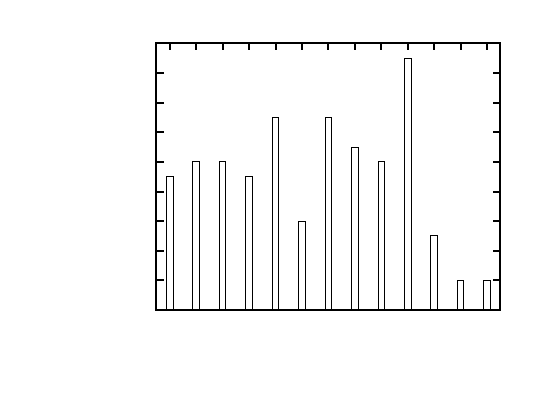
\includegraphics{DCPT-num-deltas-plot}}%
    \gplfronttext
  \end{picture}%
\endgroup

        \caption{Speedup using the DCPT prefetcher with 98 entries, and 12 bits for each delta.}
        \label{figure:dcpt-num-deltas}
    \end{centering}
\end{figure}

\begin{figure}[h]
    \begin{centering}
        % GNUPLOT: LaTeX picture with Postscript
\begingroup
  \makeatletter
  \providecommand\color[2][]{%
    \GenericError{(gnuplot) \space\space\space\@spaces}{%
      Package color not loaded in conjunction with
      terminal option `colourtext'%
    }{See the gnuplot documentation for explanation.%
    }{Either use 'blacktext' in gnuplot or load the package
      color.sty in LaTeX.}%
    \renewcommand\color[2][]{}%
  }%
  \providecommand\includegraphics[2][]{%
    \GenericError{(gnuplot) \space\space\space\@spaces}{%
      Package graphicx or graphics not loaded%
    }{See the gnuplot documentation for explanation.%
    }{The gnuplot epslatex terminal needs graphicx.sty or graphics.sty.}%
    \renewcommand\includegraphics[2][]{}%
  }%
  \providecommand\rotatebox[2]{#2}%
  \@ifundefined{ifGPcolor}{%
    \newif\ifGPcolor
    \GPcolorfalse
  }{}%
  \@ifundefined{ifGPblacktext}{%
    \newif\ifGPblacktext
    \GPblacktexttrue
  }{}%
  % define a \g@addto@macro without @ in the name:
  \let\gplgaddtomacro\g@addto@macro
  % define empty templates for all commands taking text:
  \gdef\gplbacktext{}%
  \gdef\gplfronttext{}%
  \makeatother
  \ifGPblacktext
    % no textcolor at all
    \def\colorrgb#1{}%
    \def\colorgray#1{}%
  \else
    % gray or color?
    \ifGPcolor
      \def\colorrgb#1{\color[rgb]{#1}}%
      \def\colorgray#1{\color[gray]{#1}}%
      \expandafter\def\csname LTw\endcsname{\color{white}}%
      \expandafter\def\csname LTb\endcsname{\color{black}}%
      \expandafter\def\csname LTa\endcsname{\color{black}}%
      \expandafter\def\csname LT0\endcsname{\color[rgb]{1,0,0}}%
      \expandafter\def\csname LT1\endcsname{\color[rgb]{0,1,0}}%
      \expandafter\def\csname LT2\endcsname{\color[rgb]{0,0,1}}%
      \expandafter\def\csname LT3\endcsname{\color[rgb]{1,0,1}}%
      \expandafter\def\csname LT4\endcsname{\color[rgb]{0,1,1}}%
      \expandafter\def\csname LT5\endcsname{\color[rgb]{1,1,0}}%
      \expandafter\def\csname LT6\endcsname{\color[rgb]{0,0,0}}%
      \expandafter\def\csname LT7\endcsname{\color[rgb]{1,0.3,0}}%
      \expandafter\def\csname LT8\endcsname{\color[rgb]{0.5,0.5,0.5}}%
    \else
      % gray
      \def\colorrgb#1{\color{black}}%
      \def\colorgray#1{\color[gray]{#1}}%
      \expandafter\def\csname LTw\endcsname{\color{white}}%
      \expandafter\def\csname LTb\endcsname{\color{black}}%
      \expandafter\def\csname LTa\endcsname{\color{black}}%
      \expandafter\def\csname LT0\endcsname{\color{black}}%
      \expandafter\def\csname LT1\endcsname{\color{black}}%
      \expandafter\def\csname LT2\endcsname{\color{black}}%
      \expandafter\def\csname LT3\endcsname{\color{black}}%
      \expandafter\def\csname LT4\endcsname{\color{black}}%
      \expandafter\def\csname LT5\endcsname{\color{black}}%
      \expandafter\def\csname LT6\endcsname{\color{black}}%
      \expandafter\def\csname LT7\endcsname{\color{black}}%
      \expandafter\def\csname LT8\endcsname{\color{black}}%
    \fi
  \fi
  \setlength{\unitlength}{0.0500bp}%
  \begin{picture}(5040.00,3528.00)%
    \gplgaddtomacro\gplbacktext{%
      \csname LTb\endcsname%
      \put(1210,704){\makebox(0,0)[r]{\strut{} 1.017}}%
      \put(1210,988){\makebox(0,0)[r]{\strut{} 1.018}}%
      \put(1210,1273){\makebox(0,0)[r]{\strut{} 1.019}}%
      \put(1210,1557){\makebox(0,0)[r]{\strut{} 1.02}}%
      \put(1210,1841){\makebox(0,0)[r]{\strut{} 1.021}}%
      \put(1210,2126){\makebox(0,0)[r]{\strut{} 1.022}}%
      \put(1210,2410){\makebox(0,0)[r]{\strut{} 1.023}}%
      \put(1210,2694){\makebox(0,0)[r]{\strut{} 1.024}}%
      \put(1210,2979){\makebox(0,0)[r]{\strut{} 1.025}}%
      \put(1210,3263){\makebox(0,0)[r]{\strut{} 1.026}}%
      \put(1578,484){\makebox(0,0){\strut{}90}}%
      \put(2049,484){\makebox(0,0){\strut{}98}}%
      \put(2521,484){\makebox(0,0){\strut{}120}}%
      \put(2992,484){\makebox(0,0){\strut{}140}}%
      \put(3464,484){\makebox(0,0){\strut{}160}}%
      \put(3936,484){\makebox(0,0){\strut{}180}}%
      \put(4407,484){\makebox(0,0){\strut{}196}}%
      \put(176,1983){\rotatebox{-270}{\makebox(0,0){\strut{}Speedup}}}%
      \put(2992,154){\makebox(0,0){\strut{}Number of entries in the table}}%
    }%
    \gplgaddtomacro\gplfronttext{%
    }%
    \gplbacktext
    \put(0,0){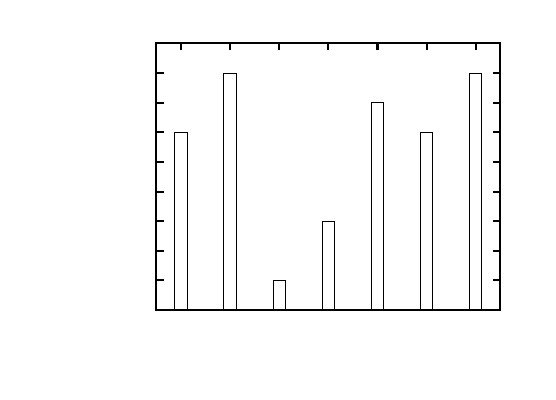
\includegraphics{DCPT-table-size-plot}}%
    \gplfronttext
  \end{picture}%
\endgroup

        \caption{Speedup using the DCPT prefetcher with 19 deltas per entry, and 12 bits for each delta.}
        \label{figure:dcpt-table-size}
    \end{centering}
\end{figure}

\begin{figure}[h]
    \begin{centering}
        % GNUPLOT: LaTeX picture with Postscript
\begingroup
  \makeatletter
  \providecommand\color[2][]{%
    \GenericError{(gnuplot) \space\space\space\@spaces}{%
      Package color not loaded in conjunction with
      terminal option `colourtext'%
    }{See the gnuplot documentation for explanation.%
    }{Either use 'blacktext' in gnuplot or load the package
      color.sty in LaTeX.}%
    \renewcommand\color[2][]{}%
  }%
  \providecommand\includegraphics[2][]{%
    \GenericError{(gnuplot) \space\space\space\@spaces}{%
      Package graphicx or graphics not loaded%
    }{See the gnuplot documentation for explanation.%
    }{The gnuplot epslatex terminal needs graphicx.sty or graphics.sty.}%
    \renewcommand\includegraphics[2][]{}%
  }%
  \providecommand\rotatebox[2]{#2}%
  \@ifundefined{ifGPcolor}{%
    \newif\ifGPcolor
    \GPcolorfalse
  }{}%
  \@ifundefined{ifGPblacktext}{%
    \newif\ifGPblacktext
    \GPblacktexttrue
  }{}%
  % define a \g@addto@macro without @ in the name:
  \let\gplgaddtomacro\g@addto@macro
  % define empty templates for all commands taking text:
  \gdef\gplbacktext{}%
  \gdef\gplfronttext{}%
  \makeatother
  \ifGPblacktext
    % no textcolor at all
    \def\colorrgb#1{}%
    \def\colorgray#1{}%
  \else
    % gray or color?
    \ifGPcolor
      \def\colorrgb#1{\color[rgb]{#1}}%
      \def\colorgray#1{\color[gray]{#1}}%
      \expandafter\def\csname LTw\endcsname{\color{white}}%
      \expandafter\def\csname LTb\endcsname{\color{black}}%
      \expandafter\def\csname LTa\endcsname{\color{black}}%
      \expandafter\def\csname LT0\endcsname{\color[rgb]{1,0,0}}%
      \expandafter\def\csname LT1\endcsname{\color[rgb]{0,1,0}}%
      \expandafter\def\csname LT2\endcsname{\color[rgb]{0,0,1}}%
      \expandafter\def\csname LT3\endcsname{\color[rgb]{1,0,1}}%
      \expandafter\def\csname LT4\endcsname{\color[rgb]{0,1,1}}%
      \expandafter\def\csname LT5\endcsname{\color[rgb]{1,1,0}}%
      \expandafter\def\csname LT6\endcsname{\color[rgb]{0,0,0}}%
      \expandafter\def\csname LT7\endcsname{\color[rgb]{1,0.3,0}}%
      \expandafter\def\csname LT8\endcsname{\color[rgb]{0.5,0.5,0.5}}%
    \else
      % gray
      \def\colorrgb#1{\color{black}}%
      \def\colorgray#1{\color[gray]{#1}}%
      \expandafter\def\csname LTw\endcsname{\color{white}}%
      \expandafter\def\csname LTb\endcsname{\color{black}}%
      \expandafter\def\csname LTa\endcsname{\color{black}}%
      \expandafter\def\csname LT0\endcsname{\color{black}}%
      \expandafter\def\csname LT1\endcsname{\color{black}}%
      \expandafter\def\csname LT2\endcsname{\color{black}}%
      \expandafter\def\csname LT3\endcsname{\color{black}}%
      \expandafter\def\csname LT4\endcsname{\color{black}}%
      \expandafter\def\csname LT5\endcsname{\color{black}}%
      \expandafter\def\csname LT6\endcsname{\color{black}}%
      \expandafter\def\csname LT7\endcsname{\color{black}}%
      \expandafter\def\csname LT8\endcsname{\color{black}}%
    \fi
  \fi
  \setlength{\unitlength}{0.0500bp}%
  \begin{picture}(5040.00,3528.00)%
    \gplgaddtomacro\gplbacktext{%
      \csname LTb\endcsname%
      \put(1210,704){\makebox(0,0)[r]{\strut{} 0.995}}%
      \put(1210,1070){\makebox(0,0)[r]{\strut{} 1}}%
      \put(1210,1435){\makebox(0,0)[r]{\strut{} 1.005}}%
      \put(1210,1801){\makebox(0,0)[r]{\strut{} 1.01}}%
      \put(1210,2166){\makebox(0,0)[r]{\strut{} 1.015}}%
      \put(1210,2532){\makebox(0,0)[r]{\strut{} 1.02}}%
      \put(1210,2897){\makebox(0,0)[r]{\strut{} 1.025}}%
      \put(1210,3263){\makebox(0,0)[r]{\strut{} 1.03}}%
      \put(1617,484){\makebox(0,0){\strut{}7}}%
      \put(2167,484){\makebox(0,0){\strut{}11}}%
      \put(2717,484){\makebox(0,0){\strut{}12}}%
      \put(3268,484){\makebox(0,0){\strut{}13}}%
      \put(3818,484){\makebox(0,0){\strut{}17}}%
      \put(4368,484){\makebox(0,0){\strut{}28}}%
      \put(176,1983){\rotatebox{-270}{\makebox(0,0){\strut{}Speedup}}}%
      \put(2992,154){\makebox(0,0){\strut{}Bits per delta}}%
    }%
    \gplgaddtomacro\gplfronttext{%
    }%
    \gplbacktext
    \put(0,0){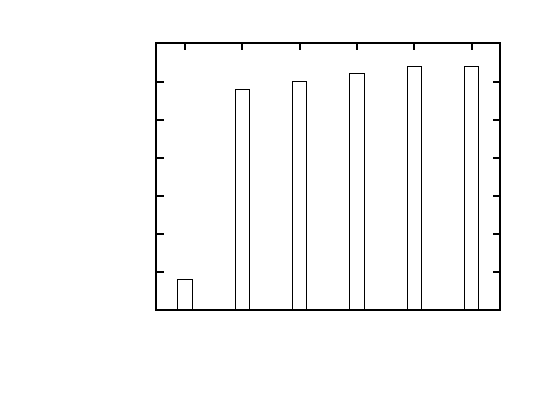
\includegraphics{DCPT-delta-bits-plot}}%
    \gplfronttext
  \end{picture}%
\endgroup

        \caption{Speedup using the DCPT prefetcher with 98 entries, and 19 deltas per entry.}
        \label{figure:dcpt-delta-bits}
    \end{centering}
\end{figure}

We obtain the best results with 98 or 196 entries in the table. In order to save size, further simulations are therefore done with 98 entries. The simulations above clearly shows that the optimal number of deltas per entry is 35. The number of bits per delta needs to be at least 11, but the performance is best with 17 or more bits per delta. 
\todo[inline]{Christian; refs below are not working, you fix? -I}
For further optimization, we combine the parameter values that give the best preformance and additionally test them with some minor variations. These results are shown in table \ref{tab:numdelta} to \ref{tab:deltabits}


\begin{table}[h]
\centering
\label{tab:numdelta}
\begin{tabular}{|l|l|l|l|l|l|l|}
\hline
32    & 33    & 34    & \textbf{35}    & 36    & 37    & 38    \\ \hline
1.028 & 1.029 & 1.029 & \textbf{1.033} & 1.027 & 1.028 & 1.027 \\ \hline
\end{tabular}
\smallskip
\caption{Number of deltas}
\end{table}


\begin{table}[h]
\centering
\label{tab:tablesize}
\begin{tabular}{|l|l|l|l|l|l|l|}
\hline
95    & 96    & 97    & \textbf{98}    & 99    & 100   & 101   \\ \hline
1.020 & 1.017 & 1.025 & \textbf{1.033} & 1.026 & 1.015 & 1.021 \\ \hline
\end{tabular}
\smallskip
\caption{Table length}
\end{table}


\begin{table}[h]
\centering
\label{tab:deltabits}
\begin{tabular}{|l|l|l|l|l|}
\hline
\textbf{12}    & 13    & 14    & 15    & 16    \\ \hline
\textbf{1.033} & 1.026 & 1.028 & 1.029 & 1.028 \\ \hline
\end{tabular}
\smallskip
\caption{Bits per delta}
\end{table}

None of the variations proved better than the original one.

\todo[inline]{The results goes here.
\\
- Show that your scheme works\\
- Compare to other schemes that do the same thing. Hopefully you are better, but you need to compare anyway\\
Trick: “Oracle Scheme”\\
- Uses “perfect” information to create an upper bound on the
performance of a class of schemes\\
- Prefetching: Best case is that all L2 accesses are hits\\
Sensitivity analysis: \\
- Check the impact of model assumptions on your
scheme}

\begin{figure}[h]
    \begin{centering}
        \input{benchmarks-plot}
        \caption{Speedup on the individual benchmarks for the TS and DCPT configurations with highest average speedup.}
        \label{figure:benchmarks-plot}
    \end{centering}
\end{figure}

Figure \ref{figure:benchmarks-plot} shows the results from each of the spec 2000 benchmarks for both TS and DCPT with optmial parameter values.
